\documentclass[12pt,a4paper]{article}
\usepackage[margin=1in]{geometry}
\usepackage{iftex}
\ifPDFTeX
  \usepackage[T1]{fontenc}
  \usepackage{newtxtext,newtxmath}
\else
  \usepackage{fontspec}
  % Use the requested Windows fonts when available, with portable
  % TeX Live fallbacks for GitHub Actions and other Linux environments.
  \IfFontExistsTF{Times New Roman}
    {\setmainfont{Times New Roman}}
    {\setmainfont{TeX Gyre Termes}}
  \IfFontExistsTF{Arial}
    {\setsansfont{Arial}}
    {\setsansfont{TeX Gyre Heros}}
  \IfFontExistsTF{Courier New}
    {\setmonofont{Courier New}}
    {\setmonofont{TeX Gyre Cursor}}
\fi
\usepackage{microtype}
\usepackage{amsmath,amssymb}
\usepackage{booktabs,longtable,tabularx,array}
\usepackage{enumitem}
\usepackage{xcolor}
\usepackage{float}
\usepackage{graphicx}
\usepackage{listings}
\usepackage{hyperref}
\usepackage{caption}
\usepackage{setspace}
\usepackage{titlesec}
\usepackage{ragged2e}
\definecolor{deepgreen}{HTML}{0D6657}
\definecolor{codegray}{HTML}{F4F6F5}
\hypersetup{colorlinks=true,linkcolor=deepgreen,citecolor=deepgreen,urlcolor=deepgreen,pdftitle={DeepGene v1: Evidence-Aware SCN1A Variant Research},pdfauthor={Deepak Pandey}}
\setlist{nosep,leftmargin=*}
\setlength{\parindent}{0pt}
\setlength{\parskip}{5pt}
\setstretch{1.5}
\justifying
\setlength{\emergencystretch}{3em}
\raggedbottom
\titleformat{\section}{\normalfont\bfseries\fontsize{16}{19.2}\selectfont}{\thesection}{1em}{}
\titleformat{\subsection}{\normalfont\bfseries\fontsize{14}{16.8}\selectfont}{\thesubsection}{1em}{}
\titleformat{\subsubsection}{\normalfont\bfseries\fontsize{14}{16.8}\selectfont}{\thesubsubsection}{1em}{}
\titlespacing*{\section}{0pt}{18pt}{8pt}
\titlespacing*{\subsection}{0pt}{14pt}{6pt}
\titlespacing*{\subsubsection}{0pt}{12pt}{5pt}
\renewcommand{\arraystretch}{1.15}
\newcommand{\code}[1]{\nolinkurl{#1}}
\newcommand{\project}{\textsc{DeepGene}}
\setlength{\fboxsep}{10pt}
\setlength{\fboxrule}{0.8pt}
\lstset{basicstyle=\ttfamily\small,backgroundcolor=\color{codegray},frame=single,breaklines=true,columns=fullflexible,showstringspaces=false}

\title{\textbf{\fontsize{16}{19.2}\selectfont DeepGene v1: Evidence-Aware SCN1A Variant Research}}
\author{Deepak Pandey\\\thanks{Correspondence: \href{mailto:deepakpandeytm@gamil.com}{deepakpandeytm@gamil.com}}}
\date{Version 1.0\\\today}

\begin{document}
\maketitle

\begin{abstract}
\textbf{Background:} SCN1A variant research requires evidence from clinical submissions, phenotype descriptions, genomic representations, functional assays, and computational annotations. These sources have different meanings and should not be collapsed into one unqualified prediction. \textbf{Objective:} We present DeepGene v1, a local-first research framework for preserving, analysing, and communicating SCN1A variant evidence while separating annotations, submitted classifications, experimental labels, and model outputs. \textbf{Methods:} The framework combines a source-preserving ClinVar pipeline, SQLite evidence storage, quality-control analysis, transparent features, leakage audits, three research-only functional-effect branches, AlphaMissense annotation ingestion, and a local browser dashboard with conversational exploration. \textbf{Results:} The current evidence snapshot contains 5,381 unique SCN1A variants, 10,696 representations, and 10,696 ClinVar records. A Generation-2 functional source contains 375 rows; after 40 exact overlaps are removed, 335 rows remain. A separate SCN1A supplementary dataset contributes 40 explicit labels, comprising 36 LOF and 4 GOF records. Its internal candidate reports ROC--AUC 0.750 and balanced accuracy 0.718. A 19,233-row AlphaMissense table is accepted as annotation evidence and does not trigger LOF/GOF retraining. \textbf{Conclusion:} DeepGene v1 is a reproducible research foundation, not a clinical decision system. Conversation is not silently treated as learning, annotation is not treated as ground truth, and exploratory performance is not presented as clinical validation.
\end{abstract}

\textbf{Keywords:} SCN1A; ClinVar; epilepsy; variant evidence; functional assay; LOF; GOF; AlphaMissense; machine learning; reproducibility

\section{Introduction}
Genomic variant interpretation is an evidence-integration problem rather than a single-model classification problem. A variant may have several genomic representations, multiple submitted interpretations, phenotype descriptions, and functional evidence of different quality. For \emph{SCN1A}, a voltage-gated sodium-channel gene associated with epilepsy and neurodevelopmental disorders, functional effects and clinical phenotypes are related but not interchangeable.

A research system must therefore distinguish what evidence is present from what target is being modelled. Reproducing a ClinVar assertion is not the same as predicting an independently reviewed clinical outcome. Similarly, an AlphaMissense score is a computational annotation, not an experimental LOF/GOF label.

DeepGene v1 was developed around this distinction. It preserves source evidence, separates biological identity from genomic representation, records transformations in scripts and manifests, and exposes uncertainty in both reports and the local dashboard. The framework provides conversational continuity through local retrieval-style memory, but it does not automatically update model parameters from ordinary conversation.

The version-one contributions are:
\begin{enumerate}
\item a provenance-aware SCN1A evidence layer and relational database;
\item descriptive analysis of classification, review status, phenotype coverage, and representation quality;
\item a policy separating evidence features, annotations, and target labels;
\item leakage-aware LOF/GOF functional-model experiments;
\item a local dashboard and Data Lab for controlled ingestion; and
\item a reproducible release record with artifacts, results, and limitations.
\end{enumerate}

\section{Related work and biological context}
ClinVar is a public archive of submitted interpretations of clinically relevant variants \cite{clinvar}. Its records differ in review status, submitter count, asserted significance, and conflict; therefore a ClinVar-derived dataset must preserve these fields rather than treating each record as an equally reliable independent label.

Functional characterization provides a complementary evidence channel. Brunklaus et al. demonstrated the value of experimental information for SCN1A interpretation \cite{brunklaus}. DeepGene uses explicit labels from the accompanying public material while retaining ambiguous, mixed, and insufficient-data rows outside the binary experiment. The Generation-2 branch uses a sodium-channel functional source represented in the project as SCION data \cite{scion}. AlphaMissense provides a separate computational annotation channel \cite{alphamissense}; its score is not promoted to experimental truth. Phenotype terminology can later be normalized using resources such as the Human Phenotype Ontology \cite{hpo}.

\section{Materials and methods}
\subsection{Scope and safety boundary}
DeepGene v1 is a local research framework. It does not diagnose disease, estimate patient risk, assign a clinical pathogenicity category, recommend treatment, or authorize clinical action. Model outputs are research candidates for hypothesis generation and pipeline development. Clinical use would require independent datasets, expert review, calibration, prospective validation, ethical oversight, and applicable regulatory assessment.

The system distinguishes:
\begin{enumerate}
\item \textbf{Conversational context:} saved local turns used for retrieval-style continuity;
\item \textbf{Annotation ingestion:} validated tables stored as evidence or metadata; and
\item \textbf{Model retraining:} controlled retraining from explicitly supported, validated labels.
\end{enumerate}
Ordinary conversation, ClinVar prose, and AlphaMissense scores are not automatically converted into training labels.

\subsection{Software architecture}
Python performs ingestion, database operations, analysis, and model training. SQLite stores structured evidence. pandas and scikit-learn support table processing and modelling. A standard-library HTTP server with HTML, CSS, and JavaScript provides the local interface. The external language-model provider is optional. The architecture is:
\begin{center}
\fcolorbox{deepgreen}{codegray}{\begin{minipage}{0.86\linewidth}
\centering
\textbf{DeepGene v1 system architecture}\\[6pt]
\begin{tabular}{c}
\textbf{Source-preserved data}\\
$\downarrow$\\
\textbf{Validated tables and SQLite evidence store}\\
$\downarrow$\\
\textbf{Quality control and feature policy}\\
$\downarrow$\\
\textbf{Research candidates, annotations, and conversation}
\end{tabular}
\end{minipage}}
\end{center}

\subsection{Data sources and provenance}
Source files, processing scripts, manifests, normalized tables, model artifacts, and reports are retained in the repository. Table~\ref{tab:data} summarizes the principal assets.

\begin{table}[H]
\centering
\small
\caption{Principal DeepGene v1 data assets.}
\label{tab:data}
\begin{tabularx}{\linewidth}{p{0.32\linewidth}p{0.22\linewidth}X}
\toprule
Asset & Role & v1 treatment\\
\midrule
SCN1A ClinVar extraction and variant summary & Clinical evidence & Source-preserved submissions; not assumed to be an independent adjudicated label set.\\
SCION-derived functional table & Cross-gene functional data & Harmonized for LOF/GOF research benchmarking after overlap checks.\\
SCN1A supplementary workbook & Gene-specific functional data & Only explicit binary LOF/GOF rows used for the candidate.\\
AlphaMissense gene/transcript table & Computational annotation & Stored as annotation; not experimental LOF/GOF truth.\\
Local conversation memory & User context & Retrieval-style continuity only; excluded from training and public release.\\
\bottomrule
\end{tabularx}
\end{table}

\subsection{ClinVar representation and database}
The source-preserved ClinVar inputs include \code{data/raw/SCN1A\_clinvar.tsv} and \code{data/raw/variant\_summary.txt.gz}; the cleaned table is \code{data/processed/SCN1A\_clinvar\_clean.csv}. The SQLite database is \code{data/database/scn1a.db}. Its core relationship is:
\begin{verbatim}
genes
  └── variants
        ├── variant_representations
        └── clinvar_records
\end{verbatim}
The \code{variants} table stores biological identifiers. \code{variant\_representations} stores assembly, coordinates, alleles, and dbSNP identifiers. \code{clinvar\_records} stores clinical significance, review status, submitter count, and phenotype descriptions. This prevents a representation from being mistaken for an independent biological observation.

\subsection{Quality control and evidence features}
Numbered analysis scripts calculate variant counts, clinical-significance distributions, review context, phenotype coverage, assembly and coordinate quality, dbSNP coverage, available prioritization signals, and leakage-audit outputs. Missing evidence is not treated as an assessed negative. The engineered table is \code{data/processed/deepgene\_evidence\_v1.csv}; the transparent baseline is \code{data/processed/deepgene\_baseline\_v1.csv}. Candidate feature groups include clinical-significance counts, submitter and review context, conflict indicators, phenotype availability, assembly quality, coordinates, dbSNP representation, and HGVS availability.

\subsection{Label policy and leakage control}
A feature that directly contains a target assertion can measure reconstruction rather than independent prediction. Using ClinVar clinical-significance text to predict the same ClinVar classification would not establish external validity. The project therefore uses overlap checks, feature-policy files, source manifests, and leakage audits:
\begin{equation}
\text{evidence used for prioritization} \ne \text{labels used for independent evaluation}.
\end{equation}
The Dravet branch remains blocked because reviewed Dravet labels are unavailable. Required fields are \code{variant\_key}, \code{dravet\_label}, \code{label\_source}, \code{source\_accession}, \code{cohort\_id}, and \code{reviewer\_status}; unresolved cases are not converted into negative labels.

\subsection{Functional data and models}
For an amino-acid substitution $a_1\rightarrow a_2$ at protein position $p$, the functional representation contains position, same-amino-acid status, hydropathy values and difference, charge values and difference, molecular-volume values and difference, and gene indicators. Unsupported amino-acid symbols and ambiguous functional effects are excluded from the binary experiment. The original independent branch uses 14 biological predictors and retains a three-class target (Loss, Mixed, and Gain); the Generation-2 branch adds gene indicators for cross-gene validation; and the SCN1A supplementary branch uses explicit binary LOF/GOF labels.

The Generation-2 candidate uses Gradient Boosting with logistic regression, random forest, and radial-basis SVM comparisons. Its primary evaluation is leave-one-gene-out cross-validation. The SCN1A supplementary candidate combines 40 explicit experimental rows with existing harmonized data, removes duplicate variant-label combinations, and evaluates a stratified random holdout. Metrics are balanced accuracy, ROC--AUC, macro F1, class-wise precision, recall, and support. Because datasets are small and source-dependent, values are descriptive and not clinical performance estimates.

\subsection{AlphaMissense and dashboard workflow}
The Data Lab validates the compressed AlphaMissense table, skips comment lines, detects \code{transcript\_id} and \code{mean\_am\_pathogenicity}, checks scores in $[0,1]$, and writes a normalized CSV. It is stored as annotation evidence and does not retrain the functional classifier because it contains no reviewed LOF/GOF target.

The dashboard is served by \code{app/server.py}. Research Chat answers database, model-status, learning-loop, and project-structure questions. Data Lab validates uploads and routes them to the correct ingestion path. Turns are stored in \code{data/memory/conversations.jsonl} for local retrieval-style context. The optional external provider uses \code{OPENROUTER\_API\_KEY}; without it, a local rule-based assistant remains available.

\subsection{Frontend and conversational interface}
DeepGene v1 includes a custom local browser frontend rather than a generic chat application or GitHub Copilot framework. The interface is implemented with semantic HTML, CSS, and browser JavaScript, and communicates with the Python server through JSON endpoints. This keeps the research workflow inspectable and allows the same evidence and safety policies to be used whether the answer is generated by the local rule-based assistant or the optional external language-model provider.

The Research Chat page provides a workspace summary, prompt suggestions, conversational history, model-status indicators, V2 research-priority results, a learning-loop explanation, and a visible safety boundary. The Data Lab page provides dataset-type selection, file upload, schema validation, processing feedback, and a contract describing the columns expected by functional, AlphaMissense, and clinical-label workflows. The interface is therefore Copilot-style in interaction design, but it is a project-specific research assistant and should not be described as Microsoft Copilot, GitHub Copilot, or an autonomous clinical agent.

Figure~\ref{fig:researchchat} shows the Research Chat workspace, while Figure~\ref{fig:datalab} shows the Data Lab upload and validation interface.

\begin{figure}[H]
\centering
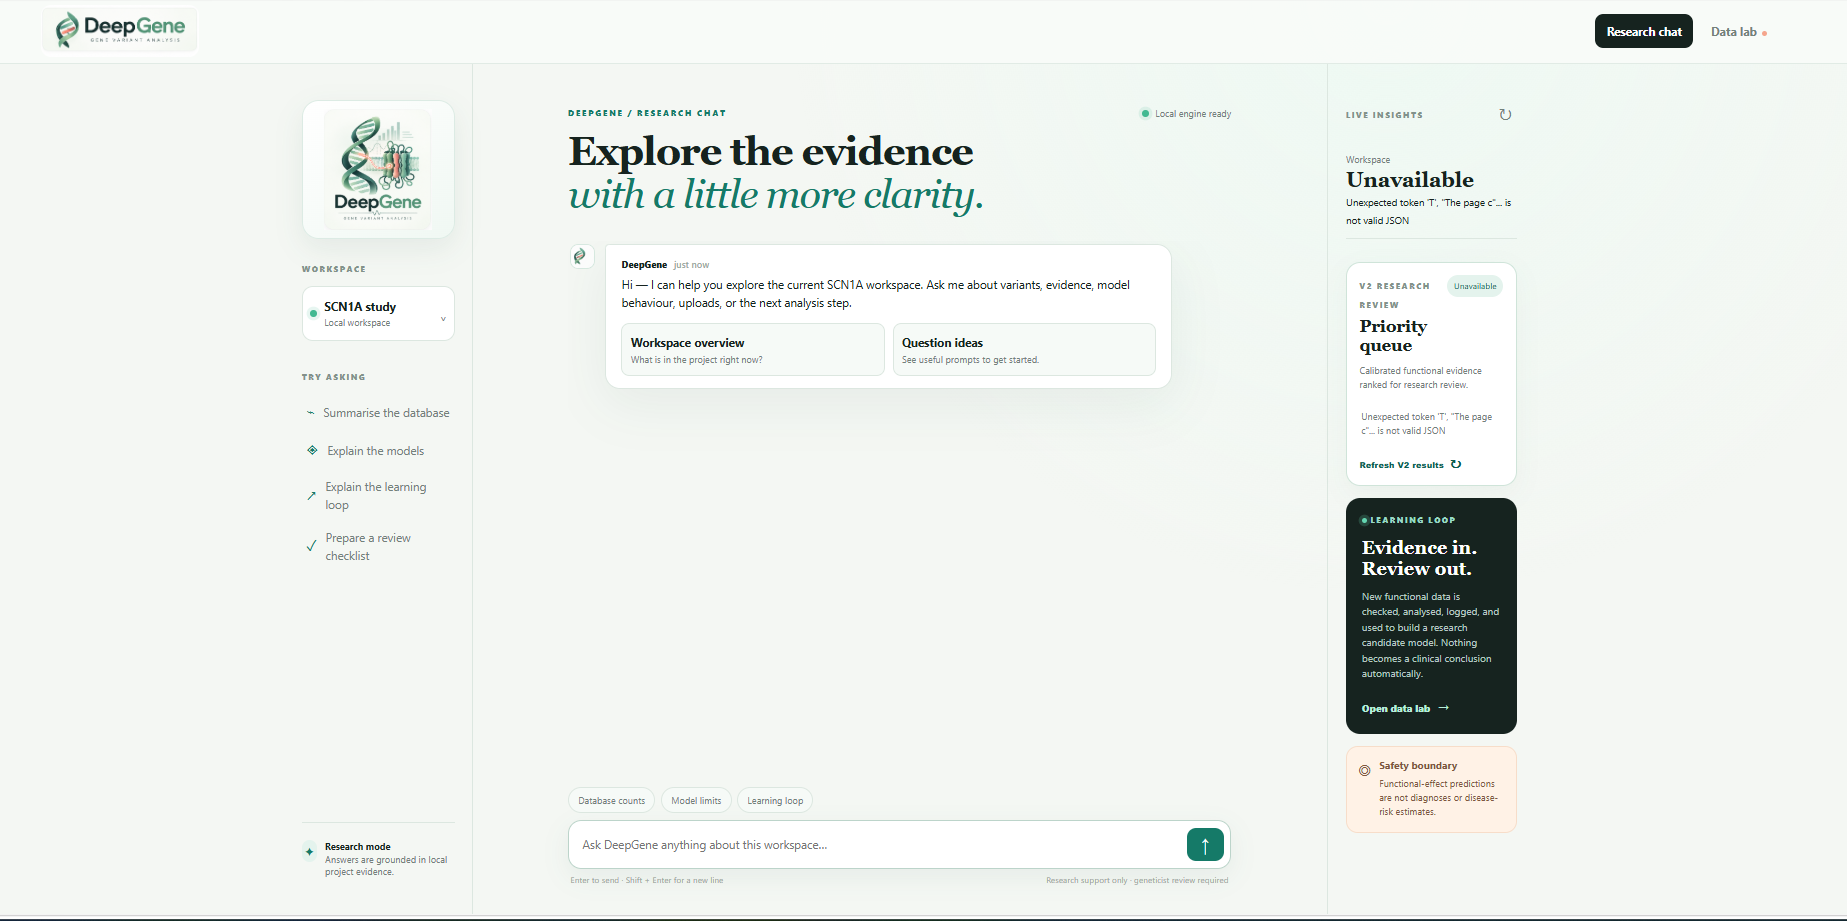
\includegraphics[width=\linewidth]{figures/deepgene-research-chat.png}
\caption{DeepGene Research Chat frontend. The page combines conversational evidence exploration with workspace status, V2 research review, learning-loop information, and a research-only safety boundary.}
\label{fig:researchchat}
\end{figure}

\begin{figure}[H]
\centering
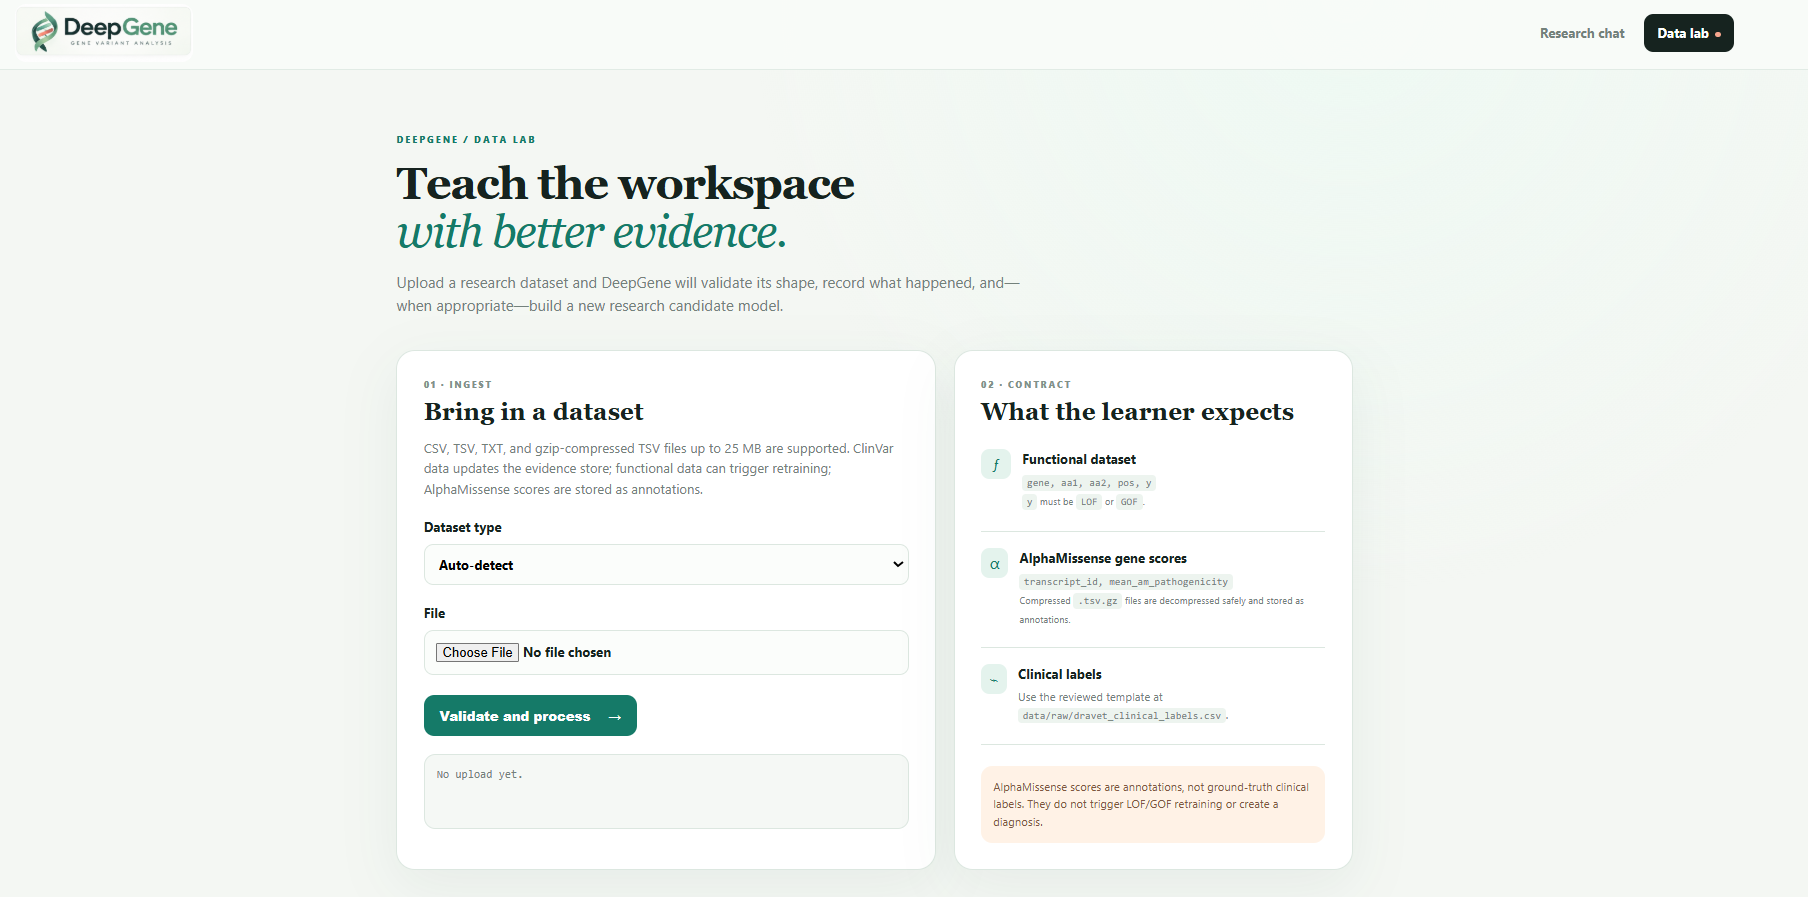
\includegraphics[width=\linewidth]{figures/deepgene-data-lab.png}
\caption{DeepGene Data Lab frontend. The page separates ingestion, dataset contracts, validation, annotation handling, and controlled retraining decisions.}
\label{fig:datalab}
\end{figure}

\section{Results}
\subsection{Graphical overview of the DeepGene workflow}
Figure~\ref{fig:graphicalabstract} summarizes the complete research workflow. DeepGene keeps source evidence, derived annotations, model outputs, and conversational context as separate products so that each result can be traced back to its origin.

\begin{figure}[H]
\centering
\fcolorbox{deepgreen}{codegray}{\begin{minipage}{0.91\linewidth}
\centering
\textbf{DeepGene evidence-to-research workflow}\\[6pt]
\begin{tabular}{c}
\textbf{Public genomic and functional sources}\\
$\downarrow$\\[-2pt]
\textbf{Source preservation and provenance manifests}\\
$\downarrow$\\[-2pt]
\textbf{Normalization, identity resolution, and quality control}\\
$\downarrow$\\[-2pt]
\textbf{Evidence store and annotation products}\\
$\downarrow$\\[-2pt]
\textbf{Leakage-controlled features and labelled research datasets}\\
$\downarrow$\\[-2pt]
\textbf{Validation, calibration, uncertainty, and error analysis}\\
$\downarrow$\\[-2pt]
\textbf{Research candidates, prioritization, and transparent communication}
\end{tabular}
\end{minipage}}
\caption{Graphical overview of the DeepGene research workflow. Conversation provides retrieval-style context and does not bypass data validation or model-governance controls.}
\label{fig:graphicalabstract}
\end{figure}

\subsection{Complete dataset summary}
Table~\ref{tab:datasetsummary} summarizes the principal data products used by the V1 baseline and V2 extension. Row counts refer to the current local snapshot and may change when upstream sources are updated.

\begin{longtable}{p{0.24\linewidth}p{0.18\linewidth}p{0.16\linewidth}p{0.31\linewidth}}
\caption{DeepGene dataset summary and scientific role.}\label{tab:datasetsummary}\\
\toprule
Dataset & Source or format & Size & Scientific role\\
\midrule
\endfirsthead
\toprule
Dataset & Source or format & Size & Scientific role\\
\midrule
\endhead
SCN1A ClinVar evidence & ClinVar extraction & 10,696 records; 5,381 variants & Submitted clinical evidence and representation analysis; not an independent gold standard.\\
Independent functional source & SCN1A functional study & 51 primary rows & Exploratory three-class functional-effect analysis.\\
Generation-2 functional source & SCION-derived table & 375 source rows; 335 after overlap removal & Cross-gene LOF/GOF research benchmarking.\\
SCN1A supplementary labels & Supplementary workbook & 40 explicit labels & Gene-specific LOF/GOF candidate development.\\
AlphaMissense annotations & Compressed gene/transcript table & 19,233 rows & Computational annotation; not experimental labels.\\
HPO staging table & Conservative exact mappings & Project-derived & Phenotype normalization and future ontology enrichment.\\
gnomAD population evidence & gnomAD v4.1.2/API & 2,901 matched representations & Population-frequency evidence with explicit matching provenance.\\
Conversation memory & Local JSONL store & User-dependent & Retrieval-style context only; excluded from model training.\\
\bottomrule
\end{longtable}

\subsection{Database coverage and representation quality}
The evidence snapshot contains one gene, 5,381 unique variants, 10,696 genomic representations, and 10,696 ClinVar records. All representations have complete reference and alternate alleles and dbSNP identifiers. Coordinates are available for 10,686 representations (99.91\%), leaving 10 without coordinates. GRCh37 is represented for 5,369 records and GRCh38 for 5,317; 5,315 representations are available in both assemblies.

\begin{table}[H]
\centering
\small
\caption{Evidence-layer counts and quality-control results.}
\label{tab:coverage}
\begin{tabular}{lr}
\toprule
Measure & Value\\
\midrule
Genes & 1\\
Unique SCN1A variants & 5,381\\
Variant representations & 10,696\\
ClinVar records & 10,696\\
dbSNP representation coverage & 10,696 (100\%)\\
Complete reference/alternate alleles & 10,696 (100\%)\\
Coordinate coverage & 10,686 (99.91\%)\\
Representations in both GRCh37 and GRCh38 & 5,315\\
GRCh37 representations & 5,369\\
GRCh38 representations & 5,317\\
\bottomrule
\end{tabular}
\end{table}

No orphan genomic representations or orphan ClinVar records were reported in the relational integrity checks. These results describe database completeness, not biological completeness of SCN1A variation.

\subsection{Clinical significance, review, and phenotype}
At the record level, the most frequent categories were uncertain significance (3,413), pathogenic (2,707), likely benign (1,575), likely pathogenic (1,269), and conflicting classifications (772). At the unique-variant level, the corresponding counts were 1,710, 1,380, 788, 637, and 386.

The unique-variant review context includes 3,741 variants with criteria from a single submitter, 1,083 with multiple submitters and no recorded conflict, 386 with conflicting classifications, 68 with no assertion criteria, 59 with no classification, and 22 with expert-panel review. There are 1,592 variants with multiple submitters.

Phenotype information is present for all 5,381 unique variants and all 10,696 records in the current parsed dataset. Frequent terms include Early-infantile developmental and epileptic encephalopathy (2,050 records), Severe myoclonic epilepsy in infancy (426), and Developmental and epileptic encephalopathy (132). Current phenotype parsing preserves descriptions but does not yet provide full ontology normalization or patient-level modelling.

\begin{table}[H]
\centering
\small
\caption{Selected record-level and unique-variant counts.}
\label{tab:clinical}
\begin{tabular}{lrr}
\toprule
Category & Records & Unique variants\\
\midrule
Uncertain significance & 3,413 & 1,710\\
Pathogenic & 2,707 & 1,380\\
Likely benign & 1,575 & 788\\
Likely pathogenic & 1,269 & 637\\
Conflicting classifications & 772 & 386\\
Pathogenic/Likely pathogenic & 426 & 213\\
Benign & 246 & 123\\
Not provided & 118 & 59\\
\bottomrule
\end{tabular}
\end{table}

\subsection{Functional-model benchmarks}
The original independent functional-effect analysis was kept separate from ClinVar pathogenicity evidence. Its primary supervised table contains 51 variants, 26 columns, and three functional classes: Loss (35), Mixed (12), and Gain (4). The 14 biological predictors are protein position and amino-acid physicochemical properties; identifiers, phenotype, inheritance, ClinVar evidence variables, and the functional target itself were excluded from the predictors. The majority-class balanced-accuracy baseline was 0.3333. Repeated stratified cross-validation produced balanced accuracy 0.2750 $\pm$ 0.0740 for logistic regression and 0.3032 $\pm$ 0.1663 for random forest. The target-permutation audit did not show unusually high performance relative to randomized labels, and no final predictive model was selected. This is an exploratory negative/insufficient finding, not evidence that the biological features have no relationship with functional effect.

The Generation-2 source contains 375 rows from nine sodium-channel genes. After removing 40 exact protein-level overlaps, 335 rows remain. Gradient Boosting achieved mean balanced accuracy $0.6368 \pm 0.1465$ in leave-one-gene-out evaluation; comparison means were 0.6144 for logistic regression, 0.6196 for random forest, and 0.5938 for radial-basis SVM. This is source-dependent and not clinical or fully independent external validation.

The SCN1A supplementary candidate uses 377 deduplicated rows and a 95-row internal holdout. ROC--AUC was 0.750 and balanced accuracy was 0.718. The underlying supplement contains only 4 explicit GOF labels and 36 LOF labels, so this result is a development signal rather than a stable generalization estimate.

\begin{table}[H]
\centering
\small
\caption{SCN1A supplementary candidate internal holdout.}
\label{tab:supplement}
\begin{tabular}{lrrrr}
\toprule
Class & Precision & Recall & F1 & Support\\
\midrule
GOF & 0.711 & 0.643 & 0.675 & 42\\
LOF & 0.737 & 0.792 & 0.764 & 53\\
\midrule
Accuracy & \multicolumn{3}{r}{0.726} & 95\\
Macro F1 & \multicolumn{3}{r}{0.719} & 95\\
\bottomrule
\end{tabular}
\end{table}

The model artifacts and reports preserve both conclusions: the original 51-variant branch did not justify selecting a final model, while the later Generation-2 and SCN1A supplement branches remain research candidates with their own validation limitations. No branch is a clinical predictor.

\subsection{Consolidated model-evaluation summary}
Table~\ref{tab:modelevaluation} places the exploratory model results beside their validation design and interpretation. The table is intentionally descriptive: a metric from an internal or source-dependent split is not equivalent to external clinical validation.

\begin{table}[H]
\centering
\small
\caption{Consolidated evaluation of DeepGene functional-model branches.}
\label{tab:modelevaluation}
\begin{tabularx}{\linewidth}{p{0.23\linewidth}p{0.20\linewidth}p{0.17\linewidth}p{0.15\linewidth}X}
\toprule
Branch & Target and data & Validation & Main result & Interpretation\\
\midrule
Independent functional & Loss/Mixed/Gain; 51 variants & Repeated stratified CV & Balanced accuracy 0.275--0.303 & Insufficient evidence to select a final model.\\
Generation-2 & LOF/GOF; 335 post-overlap rows & Leave-one-gene-out & GBM balanced accuracy $0.6368\pm0.1465$ & Source-dependent cross-gene research candidate.\\
SCN1A supplement & LOF/GOF; 377 deduplicated rows & Internal 95-row holdout & ROC--AUC 0.750; balanced accuracy 0.718 & Development signal requiring independent validation.\\
\bottomrule
\end{tabularx}
\end{table}

\subsection{Annotation ingestion and operational behaviour}
The AlphaMissense upload path normalizes 19,233 gene/transcript score rows into \code{data/processed/alphamissense\_gene\_hg38.csv} and reports \code{retrained=false}. This is scientifically correct because the file contains scores but no reviewed LOF/GOF target. The dashboard exposes health, summary, question, and upload endpoints. The external provider is optional and does not change the label policy.

\section{Discussion}
DeepGene v1 shows that a useful genomic research assistant can be built without claiming autonomous self-training. Its main result is a traceable chain from source data to database, analysis report, feature policy, model artifact, and user-facing explanation.

The evidence layer shows substantial heterogeneity. Uncertain-significance records are common, multiple submitters are present for many variants, and conflicts are measurable rather than hidden. Record-level and unique-variant counts must not be treated as interchangeable because records represent submissions whereas unique variants represent biological entities.

The functional results suggest that simple physicochemical features contain some signal for LOF/GOF separation, but variation across held-out genes indicates that performance is not uniform. The SCN1A result is useful for pipeline development, yet its internal split, small labels, and dependence on combined data prevent clinical interpretation. Future evaluation should use variant-level deduplication, cohort-aware splits, independent external data, calibration, confidence intervals, and reviewed labels.

The conversational component is intentionally narrower than autonomous self-learning. Saved text provides context but does not validate facts, assign targets, or update model parameters. Automatic self-training from unreviewed conversation would introduce label noise, privacy risks, and feedback loops. In v1, retraining is controlled by data type and validation checks.

\section{Limitations}
\begin{enumerate}
\item ClinVar submissions have heterogeneous evidence quality, review status, and possible conflict.
\item Phenotype strings are preserved but not fully normalized or modelled at patient level.
\item Population frequency, conservation, splice, structural, and patient-level genotype/phenotype evidence are incomplete.
\item Functional labels are assay- and context-dependent; LOF and GOF are not direct clinical outcomes.
\item Generation-2 evaluation is source-dependent and has limited external independence.
\item The SCN1A metric is from an internal holdout, not an external test set.
\item AlphaMissense annotations are not experimental labels and do not establish clinical pathogenicity.
\item Conversation memory can contain mistakes and is not trusted as automatic training data.
\item The Dravet outcome branch is blocked until reviewed outcome labels are supplied.
\item No v1 artifact is a diagnostic, risk, treatment, or clinical decision model.
\end{enumerate}

\subsection{Threats to validity}
Several threats affect how the reported results should be interpreted. First, source selection and dataset construction may introduce ascertainment bias because publicly available variants are not a random sample of all SCN1A variation. Second, labels originate from different assays, publications, and interpretation contexts; identical LOF or GOF labels do not necessarily represent identical biological mechanisms. Third, small class counts, especially for GOF, make point estimates unstable and widen the risk of optimistic internal results. Fourth, representations, annotations, and labels can be correlated through shared source records, creating leakage unless overlap and feature policies are enforced. Fifth, missing evidence is not missing at random: variants that are less studied may have fewer phenotype, functional, or population annotations. Sixth, the current population matching result is a coverage measurement, not evidence that unmatched variants are rare or benign. Finally, the local language-model interface can produce fluent but incorrect explanations; every scientific conclusion must therefore be checked against the stored evidence and reports.

These threats motivate the V2 controls of variant-level deduplication, source-aware and cohort-aware splits, temporal or external evaluation where feasible, calibration, uncertainty reporting, provenance tracking, and explicit human review. They also prevent the current metrics from being interpreted as clinical sensitivity, specificity, or diagnostic accuracy.

\section{Reproducibility and availability}
The repository is available at \url{https://github.com/deepakpandeymaths/Project_DeepGene}. From the project root, start the dashboard with:
\begin{lstlisting}
python app/server.py
\end{lstlisting}
It is available at \url{http://127.0.0.1:8765/}. An external provider key is optional:
\begin{lstlisting}
$env:OPENROUTER_API_KEY="your-real-key"
python app/server.py
\end{lstlisting}
Core checks and candidate rebuild:
\begin{lstlisting}
python -m py_compile app/server.py
node --check app/static/app.js
python data/ml/49_prepare_scn1a_supplement.py
python data/ml/49_train_scn1a_supplement.py
\end{lstlisting}

The version-one repository is organized into the following functional areas:
\begin{longtable}{p{0.30\linewidth}p{0.60\linewidth}}
\caption{DeepGene v1 repository areas.}\label{tab:repository}\\
\toprule
Directory & Contents\\
\midrule
\endfirsthead
\toprule
Directory & Contents\\
\midrule
\endhead
\code{app/} & Local HTTP server, API routes, Research Chat, Data Lab, frontend assets, and project logo assets.\\
\code{data/raw/} & Source-preserved ClinVar, functional, SCION, supplementary, and Dravet label-template files.\\
\code{data/processed/} & Cleaned evidence, phenotype, feature, functional, AlphaMissense, and prioritization tables.\\
\code{data/database/} & SQLite creation, loading, querying scripts, and the SCN1A evidence database.\\
\code{data/data\_analysis/} & Evidence, phenotype, feature, functional, consistency, and leakage analyses.\\
\code{data/ml/} & Dataset preparation, baseline modelling, cross-validation, audits, functional candidates, and gated Dravet workflow.\\
\code{data/ml\_results/} & Feature policies, manifests, split identifiers, model evaluation, interpretability, and error reports.\\
\code{data/model/} & Research model artifacts and model metadata.\\
\code{data/analysis\_results/} & JSON and text reports documenting intermediate and final results.\\
\code{data/uploads/} & Data Lab uploads and the upload audit log.\\
\code{data/memory/} & Local conversation context; excluded from public release and version control.\\
\code{docs/} & This version-one research manuscript.\\
\bottomrule
\end{longtable}

\begin{longtable}{p{0.39\linewidth}p{0.53\linewidth}}
\caption{Key v1 artifacts.}\\
\toprule
Artifact & Purpose\\
\midrule
\endfirsthead
\toprule
Artifact & Purpose\\
\midrule
\endhead
\code{data/database/scn1a.db} & Queryable SQLite evidence database.\\
\code{data/processed/deepgene\_v1\_final.csv} & Canonical 5,381-variant v1 dataset.\\
\code{data/processed/deepgene\_evidence\_v1.csv} & ClinVar-derived evidence features.\\
\code{data/processed/deepgene\_baseline\_v1.csv} & Transparent evidence baseline.\\
\code{data/processed/deepgene\_ml\_ready\_v1.csv} & 51-variant independent functional-effect matrix.\\
\code{data/processed/deepgene\_independent\_ml\_dataset\_v1.csv} & 56-row independent functional source before primary exclusions.\\
\code{data/processed/deepgene\_gen2\_ml\_ready\_v1.csv} & Generation-2 functional matrix.\\
\code{data/processed/deepgene\_phenotype\_normalized\_v1.csv} & Phenotype-normalized v1 table.\\
\code{data/processed/deepgene\_phenotype\_profiles\_v1.csv} & Variant-level phenotype profiles.\\
\code{data/processed/deepgene\_prioritized\_v1.csv} & Transparent research prioritization output.\\
\code{data/model/deepgene\_generation2\_gbm.pkl} & Generation-2 research candidate.\\
\code{data/processed/deepgene\_scn1a\_brunklaus\_2020\_functional.csv} & Normalized experimental labels.\\
\code{data/model/deepgene\_scn1a\_supplement\_candidate.pkl} & SCN1A research candidate.\\
\code{data/model/deepgene\_functional\_exploratory\_report.json} & Primary exploratory ML report.\\
\code{data/analysis\_results/49\_scn1a\_supplement\_model.json} & Candidate metrics and limitations.\\
\code{data/processed/alphamissense\_gene\_hg38.csv} & Normalized annotation table.\\
\code{app/server.py} & Local server, API, memory, and upload logic.\\
\code{app/static/} & Chat and Data Lab frontend.\\
\bottomrule
\end{longtable}

\subsection{GitHub repository structure}
The public GitHub repository is organized so that source data, processing
logic, derived artifacts, application code, and documentation remain
separable and auditable:
\begin{verbatim}
Project_DeepGene_2.0/
|-- app/                    server, API, frontend, and assets
|-- data/raw/               source-preserved datasets and manifests
|-- data/processed/         normalized and feature-ready tables
|-- data/database/          SQLite database scripts and database
|-- data/data_analysis/     evidence, phenotype, and QC analyses
|-- data/ml/                ML preparation, training, and audit scripts
|-- data/ml_results/        feature, split, and evaluation reports
|-- data/model/             research model artifacts and metadata
|-- data/analysis_results/  JSON and text analysis reports
|-- data/uploads/           Data Lab uploads and audit log
|-- data/memory/            local conversation context
|-- docs/                   version-one research manuscript
|-- CONTRIBUTORS.md         project acknowledgements
|-- LICENSE                 project license
`-- README.md               project documentation
\end{verbatim}

\subsection{Software project structure}
DeepGene v1 uses a modular local software structure. The data layer preserves
raw inputs and records transformations. The analysis layer produces evidence,
phenotype, representation, feature, consistency, and leakage reports. The ML
layer prepares independent targets, trains research candidates, evaluates
uncertainty and errors, and writes model artifacts. The application layer
exposes the resulting project state through a local API and browser interface.
The communication layer provides local rule-based answers and optional
OpenRouter language-model responses, while preserving the same research-only
safety policy in both modes.

The software flow is:
\begin{center}
\fbox{\begin{minipage}{0.90\linewidth}
\centering
\begin{tabular}{c}
\textbf{Data and provenance layer: raw files, manifests, and uploads}\\
$\downarrow$\\
\textbf{Processing layer: cleaning, normalization, SQLite loading}\\
$\downarrow$\\
\textbf{Analysis layer: QC, phenotype, evidence, and leakage audits}\\
$\downarrow$\\
\textbf{ML layer: target definition, features, validation, and artifacts}\\
$\downarrow$\\
\textbf{Application layer: API, dashboard, Research Chat, and Data Lab}
\end{tabular}
\end{minipage}}
\end{center}

This separation allows a new annotation table to be stored without silently
becoming a target label, and allows a model artifact to be inspected without
depending on an external language-model provider.

\section{Version-one status and future work}
Table~\ref{tab:status} records the status of the completed v1 scope.

\begin{table}[H]
\centering
\small
\caption{DeepGene v1 release status.}
\label{tab:status}
\begin{tabular}{p{0.68\linewidth}l}
\toprule
Milestone & Status\\
\midrule
ClinVar extraction and SQLite database & Complete\\
Evidence, phenotype, and QC analyses & Complete\\
Transparent evidence baseline & Complete\\
Independent functional-effect analysis & Complete\\
SCION Generation-2 functional candidate & Complete\\
SCN1A supplementary functional candidate & Complete\\
AlphaMissense annotation ingestion & Complete\\
Local dashboard, Research Chat, and memory & Complete\\
Independent clinical benchmark labels & Pending\\
Dravet clinical-outcome model & Blocked\\
External clinical validation & Pending\\
\bottomrule
\end{tabular}
\end{table}

\subsection{Version 2 future scope}
DeepGene v2 is planned as an evidence-aware and uncertainty-calibrated
research study, not as automatic clinical deployment. Its central question is
whether heterogeneous SCN1A evidence can be integrated while separately
measuring evidence completeness, conflict, uncertainty, calibration, and
research prioritization.

The planned v2 workflow is:
\begin{center}
\fbox{\begin{minipage}{0.90\linewidth}
\centering
\begin{tabular}{c}
\textbf{SCN1A variant}\\
$\downarrow$\\
\textbf{Evidence extraction and normalization}\\
$\downarrow$\\
\textbf{Evidence integration}\\
$\downarrow$\\
\textbf{Uncertainty estimation and probability calibration}\\
$\downarrow$\\
\textbf{Explainability, evidence completeness, and research prioritization}\\
$\downarrow$\\
\textbf{Expert review support}
\end{tabular}
\end{minipage}}
\end{center}

The planned research scope includes:
\begin{enumerate}
\item freezing v1 as the reproducible baseline and creating a formal SCN1A
master table and data dictionary;
\item adding population-frequency, conservation, splice, structural, broader
computational, and independently reviewed functional evidence;
\item normalizing phenotype terms with validated ontology mappings;
\item using unique-variant, cohort-aware, temporal, and external validation
splits where their data requirements are satisfied;
\item comparing transparent baselines with evidence-aware models;
\item evaluating calibration, predictive uncertainty, missing-evidence
behaviour, and conflict separately from model confidence;
\item adding explainable evidence-group contributions;
\item conducting a separate VUS prioritization experiment; and
\item testing independent expert-reviewed benchmarks, ablation studies, and
reproducible figures and tables.
\end{enumerate}

V2 will remain research decision support. A high probability will not be
interpreted as a diagnosis, and a VUS will remain a candidate for further
investigation rather than being declared pathogenic or benign. All future work
must preserve the v1 separation between evidence, annotations, labels,
predictions, and clinical claims.

\section{Version-two implementation status}
The version-two work extends the v1 evidence foundation into an auditable,
uncertainty-aware research workflow. V2 is implemented as a staged software
release on top of the frozen v1 snapshot. It does not replace the v1 data
products and does not convert the system into a clinical decision tool.

\subsection{V2 master product and modelling controls}
The V2 master table contains 5,381 SCN1A variants and is accompanied by a data
dictionary, source registry, overlap audit, grouped split identifiers, leakage
audit, evidence-completeness table, calibration reports, uncertainty outputs,
and transparent research-prioritization results. The modelling policy keeps
ClinVar assertions, functional LOF/GOF labels, computational annotations,
conversation context, and predictions as separate products.

The V2 functional workflow adds calibrated probabilities and uncertainty
estimates to the source-specific functional candidates. Research priority is
calculated from calibrated functional signal, model uncertainty, evidence gap,
and clinical conflict. This score ranks records for research review; it is not a
pathogenicity probability, disease-risk estimate, or clinical recommendation.

\subsection{V2 architecture and software flow}
The V2 architecture is organized into the following boxed flow:

\begin{center}
\fcolorbox{deepgreen}{codegray}{\begin{minipage}{0.90\linewidth}
\centering
\textbf{DeepGene V2 evidence-aware software architecture}\\[6pt]
\begin{tabular}{c}
\textbf{Source data and versioned manifests}\\
$\downarrow$\\
\textbf{Validated ingestion, normalization, and SQLite evidence store}\\
$\downarrow$\\
\textbf{Master variants, evidence completeness, overlap, and leakage audits}\\
$\downarrow$\\
\textbf{Functional models, calibration, uncertainty, and grouped validation}\\
$\downarrow$\\
\textbf{HPO and population annotation enrichment with coverage audits}\\
$\downarrow$\\
\textbf{Transparent research prioritization and explanations}\\
$\downarrow$\\
\textbf{Local API, dashboard, Research Chat, and Data Lab}
\end{tabular}
\end{minipage}}
\end{center}

This flow ensures that an annotation source can enrich an evidence profile
without silently becoming a target label. It also allows model artifacts and
reports to be inspected without requiring the optional external language-model
provider.

\subsection{Population-frequency enrichment}
Population frequency was added as annotation evidence using a local gnomAD
v4.1.2 gene export and targeted queries to the public gnomAD v4 API
\cite{gnomadapi}. The matching hierarchy is:

\begin{enumerate}
\item exact assembly, chromosome, position, reference, and alternate match;
\item allele-aware dbSNP identifier match, requiring reference and alternate
agreement;
\item targeted gnomAD API lookup for unmatched GRCh38 representations; and
\item GRCh37-to-GRCh38 coordinate conversion using a versioned UCSC chain,
followed by a second allele-validated API lookup.
\end{enumerate}

The liftover chain produced 4,184 unique GRCh38 candidates from 4,242
unmatched GRCh37 representations; 58 rows had no conversion. Only returned
variants with matching reference and alternate alleles were accepted. Failed
requests, allele conflicts, and missing API results remain explicitly
unmatched.

\begin{table}[H]
\centering
\small
\caption{Current V2 gnomAD population-evidence coverage.}
\label{tab:v2population}
\begin{tabular}{lr}
\toprule
Measure & Value\\
\midrule
ClinVar representation rows & 10,696\\
Matched representations & 2,901\\
Representation-level coverage & 27.12\%\\
V2 master variants & 5,381\\
Variants with population evidence & 1,597\\
Variant-level coverage & 29.68\%\\
Remaining unmatched representations & 7,795\\
\bottomrule
\end{tabular}
\end{table}

The current population result is partial and source-dependent. The gnomAD API
enrichment contributed 84 direct allele-consistent matches and the subsequent
liftover/API stage contributed 283 additional matches. These values are
annotation counts, not labels. The latest audit artifacts are
\code{data/analysis\_results/v2\_population\_unmatched\_audit.json},
\code{data/analysis\_results/v2\_gnomad\_api\_enrichment\_report.json},
and \code{data/analysis\_results/v2\_liftover\_gnomad\_api\_report.json}.

\subsection{V2 status and remaining work}
The following V2 components are complete or staged:

\begin{table}[H]
\centering
\small
\caption{DeepGene V2 implementation status.}
\label{tab:v2status}
\begin{tabular}{p{0.70\linewidth}l}
\toprule
Component & Status\\
\midrule
V1 baseline freeze, master table, and data dictionary & Complete\\
Grouped split, overlap, and leakage audits & Complete\\
Evidence completeness and missingness indicators & Complete\\
Functional baseline, calibration, and uncertainty & Exploratory complete\\
Research prioritization and dashboard/API integration & Exploratory complete\\
Conservative HPO staging & Annotation staging complete\\
gnomAD exact and allele-aware rsID integration & Complete with audit\\
gnomAD API enrichment & Partial\\
GRCh37-to-GRCh38 liftover enrichment & Partial\\
API retry recovery & Pending due service timeouts\\
Independent clinical validation & Pending\\
Dravet clinical-outcome model & Blocked\\
\bottomrule
\end{tabular}
\end{table}

The next technical step is checkpointed, low-rate recovery of failed API
requests, followed by evaluation of a broader regional or transcript-aware
population source. The retry process is not included in the reported coverage
until its responses are complete and allele-validated. V2 therefore reports
29.68\% as the current measured variant-level coverage rather than forcing a
target percentage.

\subsection{V2 data products and provenance}
Table~\ref{tab:v2sources} summarizes the principal V2 data products and their
scientific roles. Version and join metadata are retained with the generated
reports so that a future rerun can distinguish a changed source from a changed
processing rule.

\begin{longtable}{p{0.28\linewidth}p{0.22\linewidth}p{0.39\linewidth}}
\caption{V2 data products, provenance, and interpretation.}
\label{tab:v2sources}\\
\toprule
Product & Source or version & Role and interpretation\\
\midrule
\endfirsthead
\toprule
Product & Source or version & Role and interpretation\\
\midrule
\endhead
V2 master variant table & ClinVar-derived v1 snapshot & Canonical SCN1A identity and evidence join product; not an adjudicated clinical label set.\\
Functional evidence & SCION and SCN1A supplementary source & Source-specific LOF/GOF or functional-effect experiments; targets remain separate from ClinVar assertions.\\
AlphaMissense annotations & Gene/transcript table, 19,233 rows & Computational annotation only; no automatic retraining.\\
HPO enrichment & Official HPO release hp/releases/2026-09-01 & Exact name/synonym annotation only; unmapped and ambiguous terms remain explicit.\\
Population annotations & gnomAD v4.1.2 and public API & Allele-frequency evidence joined by validated coordinates, rsID alleles, API, and liftover paths.\\
Conversation memory & Local JSONL context & Retrieval-style context only; excluded from training and public release.\\
\bottomrule
\end{longtable}

\subsection{HPO enrichment and phenotype coverage}
The V2 phenotype workflow uses the official Human Phenotype Ontology release
\code{hp/releases/2026-09-01}. It compares normalized ClinVar phenotype terms
with HPO names and synonyms using exact matching only. No approximate string
matching, disease-name inference, or guessed ontology assignment is performed.
Among 6,707 phenotype-term rows representing 115 distinct normalized terms,
109 rows received an official exact HPO match, covering 106 of 5,381 unique
SCN1A variants. The remaining 6,598 rows remain unresolved for curated review.
All HPO rows retain \code{safe\_for\_training=0}: these annotations are not
clinical labels, pathogenicity labels, or LOF/GOF targets.

The HPO audit is stored in
\code{data/analysis\_results/v2\_hpo\_join\_audit.json}, and the normalized
annotation table is stored in
\code{data/processed/deepgene\_v2\_hpo\_annotations.csv}. This conservative
coverage is a transparent annotation baseline; it should not be interpreted as
complete phenotype coverage or as evidence that an unmatched variant lacks a
phenotype.

\subsection{Coverage accounting and uncertainty reporting}
The population result is reported at two levels because one biological variant
can have multiple genomic representations. Representation-level coverage is
the fraction of ClinVar representation rows with a validated population match.
Variant-level coverage is the fraction of master biological variants for which
at least one representation has validated population evidence. The distinction
prevents multiple coordinate rows from being mistaken for independent variants.

\begin{table}[H]
\centering
\small
\caption{Breakdown of the current population-evidence enrichment.}
\label{tab:v2coveragebreakdown}
\begin{tabular}{p{0.62\linewidth}r}
\toprule
Enrichment component & Matched rows\\
\midrule
Exact coordinate and allele matches & 1,407\\
Allele-aware rsID matches & 1,127\\
Direct gnomAD API matches & 84\\
GRCh37 liftover followed by API matching & 283\\
Total matched representations & 2,901\\
V2 variants with at least one match & 1,597\\
\bottomrule
\end{tabular}
\end{table}

The components are not interpreted as independent biological evidence sources;
they describe matching routes into the same population database. The reported
uncertainty therefore includes both model uncertainty and evidence availability.
Missing population evidence contributes an explicit missingness indicator and
does not imply rarity, benignity, or absence from the population.

\subsection{Reproducibility and software quality}
The repository retains source manifests, transformation scripts, generated
reports, model artifacts, API response logs, and regression tests. The V2
regression suite contains ten tests covering master-table integrity, functional
target separation, grouped split boundaries, leakage policy, API contracts,
population joins, and liftover coverage accounting. The application and
frontend are additionally checked with Python bytecode compilation and
JavaScript syntax validation. The primary local commands are:

\begin{lstlisting}
python -m unittest discover -s tests -p "test_v2_*.py" -v
python -m py_compile app/server.py
node --check app/static/app.js
\end{lstlisting}

The experiments are intended to be rerunnable on a local Windows or Python
environment. Exact metric reproduction requires the same source releases,
feature policies, split identifiers, model settings, and random seeds. API
responses are treated as time-sensitive external evidence and are preserved
when available.

\subsection{Ethics, privacy, and responsible AI}
DeepGene is designed as a research-support system for evidence organization
and hypothesis generation. Local conversation memory may contain sensitive
research notes and is therefore excluded from version control. API keys remain
server-side and are not included in source files or public artifacts. The
optional language-model provider receives only the request context selected by
the application; it is not used as an automatic label generator.

The system does not infer a patient's diagnosis, treatment, prognosis, or
disease risk. Human review remains necessary for interpretation of conflicting
submissions, uncertain evidence, functional assay context, and any future
clinical application. Any future clinical study would require independent
reviewed cohorts, consent and governance procedures, calibration, external
validation, and appropriate regulatory assessment.

\subsection{Structured limitations}
The main limitations are separated by layer in Table~\ref{tab:v2limits}.

\begin{table}[H]
\centering
\small
\caption{Layered limitations of DeepGene V1 and V2.}
\label{tab:v2limits}
\begin{tabular}{p{0.22\linewidth}p{0.68\linewidth}}
\toprule
Layer & Limitation\\
\midrule
Data & ClinVar submissions are heterogeneous; functional labels are small and assay-dependent; phenotype strings are not patient-level observations.\\
External evidence & Current gnomAD enrichment is partial, API responses can fail or change, and unmatched values remain unavailable.\\
Representation & Multiple assemblies and representations require careful deduplication; record counts are not independent variant counts.\\
Model & Functional candidates are source-dependent, internally evaluated, and not externally calibrated for clinical use.\\
Communication & Conversation memory can contain errors and provides context rather than validated knowledge or training labels.\\
Clinical scope & No DeepGene V1 or V2 artifact is a diagnostic, pathogenicity, risk, treatment, or clinical decision model.\\
\bottomrule
\end{tabular}
\end{table}

\section{Conclusion}
DeepGene v1 provides an inspectable foundation for SCN1A variant research, and
the V2 implementation extends that foundation with a master evidence product,
grouped validation controls, calibration, uncertainty estimation, transparent
research prioritization, and audited population-frequency enrichment. The
current population result reaches 29.68\% at the variant level after exact,
API, and liftover-assisted allele validation, while the remaining gaps and API
failures are explicitly recorded. The functional candidates and V2 priority
scores support hypothesis generation and pipeline development, but their small
datasets and limited validation preclude clinical deployment. The appropriate
next step is independently reviewed evidence followed by cohort-aware external
validation rather than unrestricted self-training.

\section*{Author contributions}
The DeepGene Research Software Project designed the software architecture, data model, analysis workflow, dashboard, model experiments, and version-one documentation.

\section*{Data and software availability}
The source code, scripts, manifests, processed research tables, model artifacts, and reports are maintained in the repository above. Third-party datasets remain subject to their original licenses and usage conditions. Local conversation memory and secrets are not part of the public release.

\begin{thebibliography}{9}
\bibitem{clinvar}
Landrum MJ, Lee JM, Benson M, et al.
ClinVar: public archive of interpretations of clinically relevant variants.
\emph{Nucleic Acids Research}. 2016;44(D1):D862--D868.
\url{https://www.ncbi.nlm.nih.gov/clinvar/intro/}

\bibitem{brunklaus}
Brunklaus A, Schorge S, Smith AD, et al.
SCN1A variants from bench to bedside---improved clinical prediction from functional characterization.
\emph{Human Mutation}. 2020;41(2):363--374.
\url{https://discovery.ucl.ac.uk/id/eprint/10091164/}

\bibitem{scion}
Bosselmann C, et al.
SCION: functional data and analysis resources for sodium-channel variants.
Source repository.
\url{https://github.com/christianbosselmann/SCION}

\bibitem{alphamissense}
Cheng J, Novati G, Pan J, et al.
Accurate proteome-wide missense variant effect prediction with AlphaMissense.
\emph{Science}. 2023;381(6664):eadg7492.
\url{https://github.com/google-deepmind/alphamissense}

\bibitem{hpo}
Köhler S, Gargano M, Matentzoglu N, et al.
The Human Phenotype Ontology in 2021.
\emph{Nucleic Acids Research}. 2021;49(D1):D1207--D1217.
\url{https://hpo.jax.org/}

\bibitem{gnomadapi}
gnomAD Browser Team.
gnomAD GraphQL API and browser data resources.
\url{https://github.com/broadinstitute/gnomad-browser/tree/main/graphql-api}

\bibitem{ucsc}
UCSC Genome Browser.
LiftOver coordinate conversion resources and hg19-to-hg38 chain files.
\url{https://hgdownload.soe.ucsc.edu/goldenPath/hg19/liftOver/}
\end{thebibliography}

\end{document}

